\section{Results}\label{sec:results}

This section presents the results of applying \texttt{GLaRe()} to our three motivating datasets --  the Glaucoma data (Section \ref{sec:glaucoma-reults}), the Proteomic Gels data (Section \ref{sec:gels-reults}) and the MNIST digits data (Section \ref{sec:mnist-reults}) -- to choose between our three built-in latent feature representation methods described in Section \ref{sec:learning-functions} -- Principal Components Analysis (PCA), the Discrete Wavelet Transform (DWT) and an autoencoder (AE).
For all three datasets, we use a tolerance level of $\epsilon = 0.05$ and attainment rate of $\alpha=0.95$ with hyperparameters and settings for the methods set at their defaults outlined in Section \ref{sec:learning-functions} unless otherwise specified.
Finally, in Section \ref{sec:sample-size-experiment}, we perform an experiment where we artificially decimate the sample size of the Glaucoma dataset to demonstrate how the optimal latent representation can depend on sample size, with more flexible empirical methods (e.g. PCA) working well when there is enough data to reliably estimate the latent features, and fixed methods (e.g. wavelets) performing better when there is not.
%the dependence of PCA and the DWT on different sample sizes.
Additional results of the case studies are presented in Appendix \ref{sec:additional-results}.

\subsection{Glaucoma Data}\label{sec:glaucoma-reults}

Figure \ref{fig:eye-results} displays the summary plot from the application of \texttt{GLaRe()} to the Glaucoma data.
PCA is the most suitable latent feature representation method for this dataset because it achieves the qualifying criterion with qualifying dimension $qd=51$, whereas DWT and AE do not achieve the qualifying criterion for $K \leq 301$.
A grid of equally-spaced values from $1$ to $301$ in increments of $10$ was used for the latent feature dimensions.
Although it was possible to use larger latent feature dimensions for the DWT and AE, it was deemed unnecessary because the qualifying criterion was achieved for PCA with a qualifying dimension $qd=51$ and is the favored method for this dataset.
PCA provides dimension reduction of $282:1$ ($T = 14400$ to $qd = 51$).
The computation times for PCA, DWT and AE were $1.3$, $0.7$ and $68.1$ minutes, respectively.


\begin{figure}
    \centering
    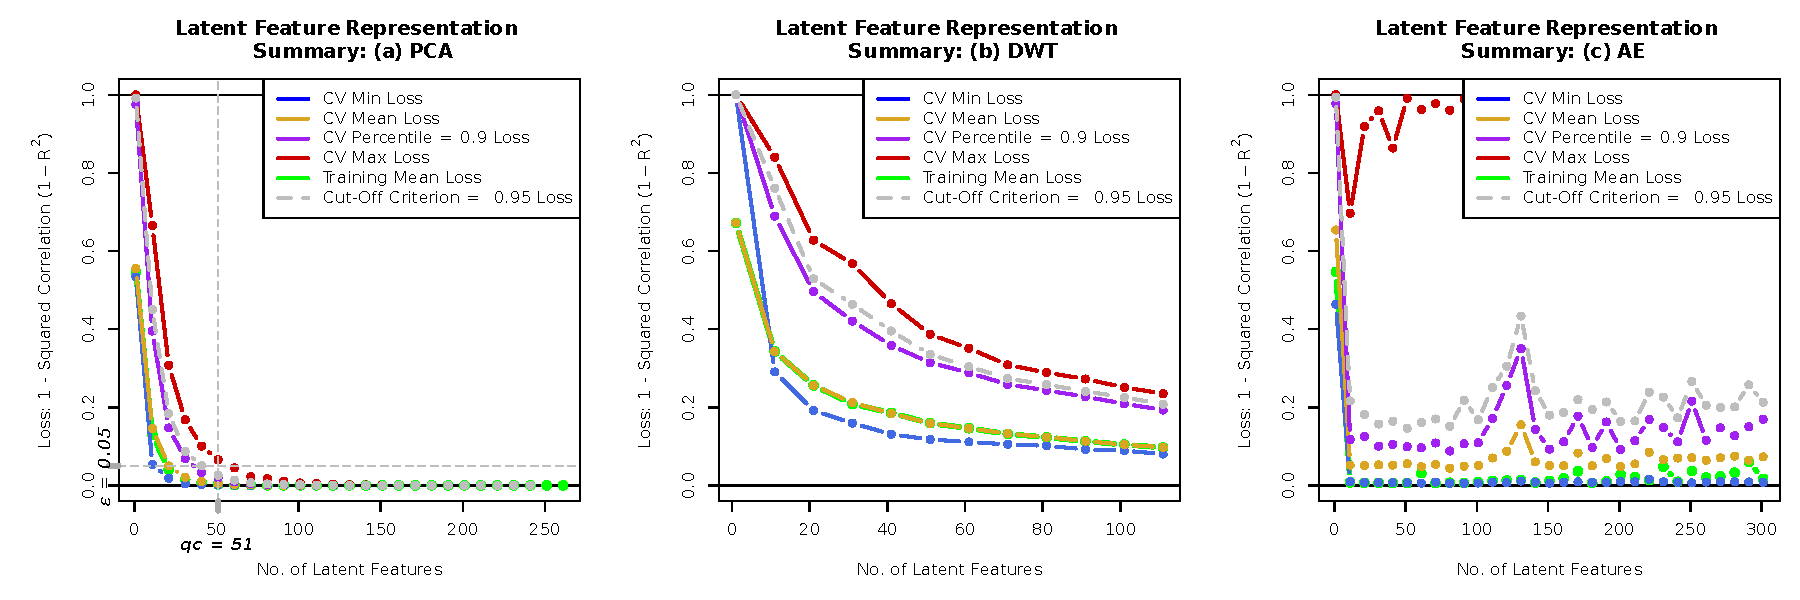
\includegraphics[width=1\textwidth]{figures/eye-results.pdf}
    \caption{Summary \texttt{GLaRe()} plot for the Glaucoma data. A grid of equally-spaced values from $1$ to $301$ in increments of $10$ was used for the latent feature dimensions. \textbf{Note}: For PCA, the maximum number of non-zero eigenvalues was $\leq361$ so only results for $K \leq 361$ are displayed on the summary plot.}
    \label{fig:eye-results}
\end{figure}

\subsection{Proteomic Gels Data}\label{sec:gels-reults}

Figure \ref{fig:gels-results} displays the summary plot from the application of \texttt{GLaRe()} to the Proteomic Gels data.
Because this dataset contains $N=53$ observations in this dataset, the maximum latent dimension for PCA is $53$ and PCA does not achieve the qualifying criterion.
In contrast, the maximum latent dimension for the DWT is not constrained and hence we run \texttt{GLaRe()} on a grid of equally-spaced values from $1$ to $8000$ in increments of $100$.
The qualifying dimension for the DWT is $qd=7801$.
{\color{purple}\textbf{Note}: Need to add AE results when run on cluster because of memory issues.}
Hence, the DWT is the favored representation method for the Proteomic Gels dataset and it provides a compression ratio of $71:1$ ($T = 556206$ to $qd = 7801$).
The computation times for PCA, DWT and AE were $0.9$, $47.6$ and {\color{purple}$X$} minutes, respectively.


\begin{figure}
    \centering
    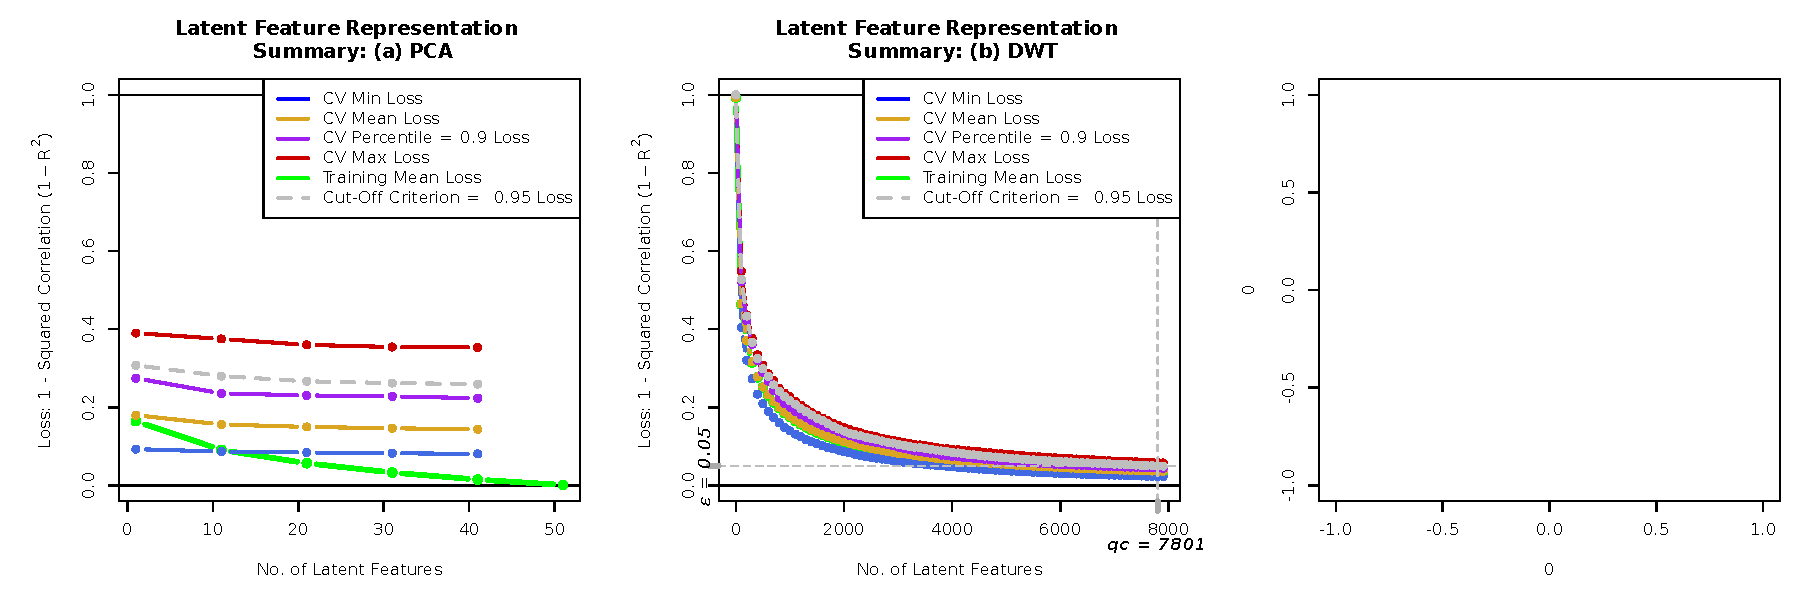
\includegraphics[width=1\linewidth]{figures/gels-results.pdf}
    \caption{Summary \texttt{GLaRe()} plot for the Proteomic Gels data. For PCA, a grid of equally-spaced values from $1$ to $53$ in increments of $10$ was used for the latent feature dimensions.
    For the DWT,  a grid of equally-spaced values from $1$ to $8000$ in increments of $10$ was used for the latent feature dimensions. {\color{purple} \textbf{Note: Need to add AE results.}}}
    \label{fig:gels-results}
\end{figure}


\subsection{MNIST Digits Data}\label{sec:mnist-reults}

Figure \ref{fig:mnist-results} displays the summary plot from the application of \texttt{GLaRe()} to the MNIST data.
A grid of equally-spaced values from $1$ to $381$ in increments of $20$ was used for the latent feature dimensions.
All three latent feature representation methods achieve the qualifying criterion within this range: $qd = 201$ for PCA, $qd = 321$ for the DWT and $qd = 101$ for the AE.
Hence, the AE is the preferred method for this dataset because it provides the most compact (i.e., smallest qd) representation.
The AE has a compression ratio of $8:1$ ($T = 784$ to $K = 101$).
The computation times for PCA, DWT and AE were $16.3$, $27.5$ and $1065.1$ minutes, respectively.

\begin{figure}
    \centering
    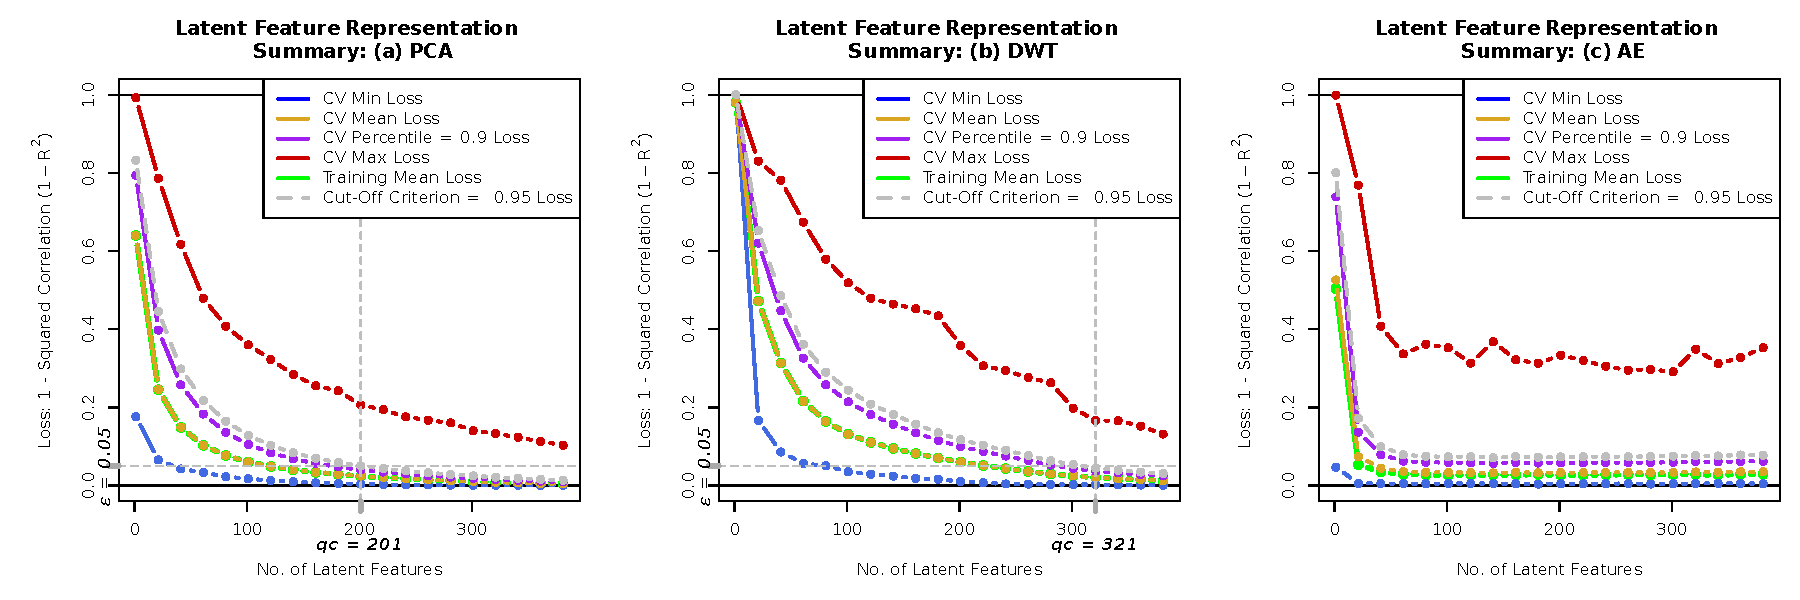
\includegraphics[width=1\textwidth]{figures/mnist-results.pdf}
    \caption{Summary \texttt{GLaRe()} plot for the MNIST data. A grid of equally-spaced values from $1$ to $381$ in increments of $20$ was used for the latent feature dimensions.}
    \label{fig:mnist-results}
\end{figure}

\subsection{Sample Size Experiment}\label{sec:sample-size-experiment}

In this section, we present the results of an experiment that demonstrates the dependence of flexible latent feature representation methods (e.g., PCA, AE) on sample size.
In PCA, the encoding and decoding transformations are learned entirely from the data, so it is highly dependent on having a sufficient sample size.
In contrast, the DWT transformation is fixed a-priori and only the ordering of the wavelet coefficients to retain is learned from the data and hence there is less reliance on sample size.
We demonstrate this concept empirically on the Glaucoma dataset. 
We start with the full dataset ($N=606$) and then sub-sample the dataset to create smaller datasets of sizes $N=153$, $N=76$ and $N=38$ respectively.
We run \texttt{GLaRe()} to compare the performance of PCA and the thresholded DWT as the sample size is successively degraded.
In all cases, because of the small sample sizes, we use leave-one-out rather than $k$-fold cross-validation.

Figure \ref{fig:eye-sample-size-results-results-01} displays the results of the experiment.
The PCA results are displayed in the top row and the DWT results are displayed in the bottom row.
As PCA can only estimate, at most, $\min(N-1, T)$ features and in this case $N<T$, we see that the maximum possible number of latent features changes as the sample size decreases.
In contrast, there is no restriction on the number of latent features for the DWT and we manually choose a maximum of $K=500$, which is sufficient to achieve the qualifying criterion (with $\epsilon=0.05$ and $\alpha=0.95$) in all four cases.
The greater reliance of PCA on sample size is reflected in Figure \ref{fig:eye-sample-size-results-results-01} in several ways.
Firstly, the displayed quantiles of the cross-validated loss distribution, in particular the maximum, $0.95$ and $0.9$ quantiles (red, grey and purple lines) increase noticeably for PCA as the sample size is decreased, but they remain stable for the DWT.
The dependence is also reflected by the separation between the training and validation mean losses (green vs. yellow lines) as sample size is decreased, which demonstrates that PCA is unable to estimate a generalizable representation when the sample size is small, even if the training loss is satisfactory.
Finally, we can achieve the qualifying criterion using the DWT in all four cases (albeit with a large number of features), but we only achieve it for PCA with sample sizes $N=306$ and $N=153$.
The experiment is subject to sampling variability induced in the sub-sampling stage, so is repeated using a different random seed in Appendix \ref{sec:additional-results}.

\begin{figure}
    \centering
    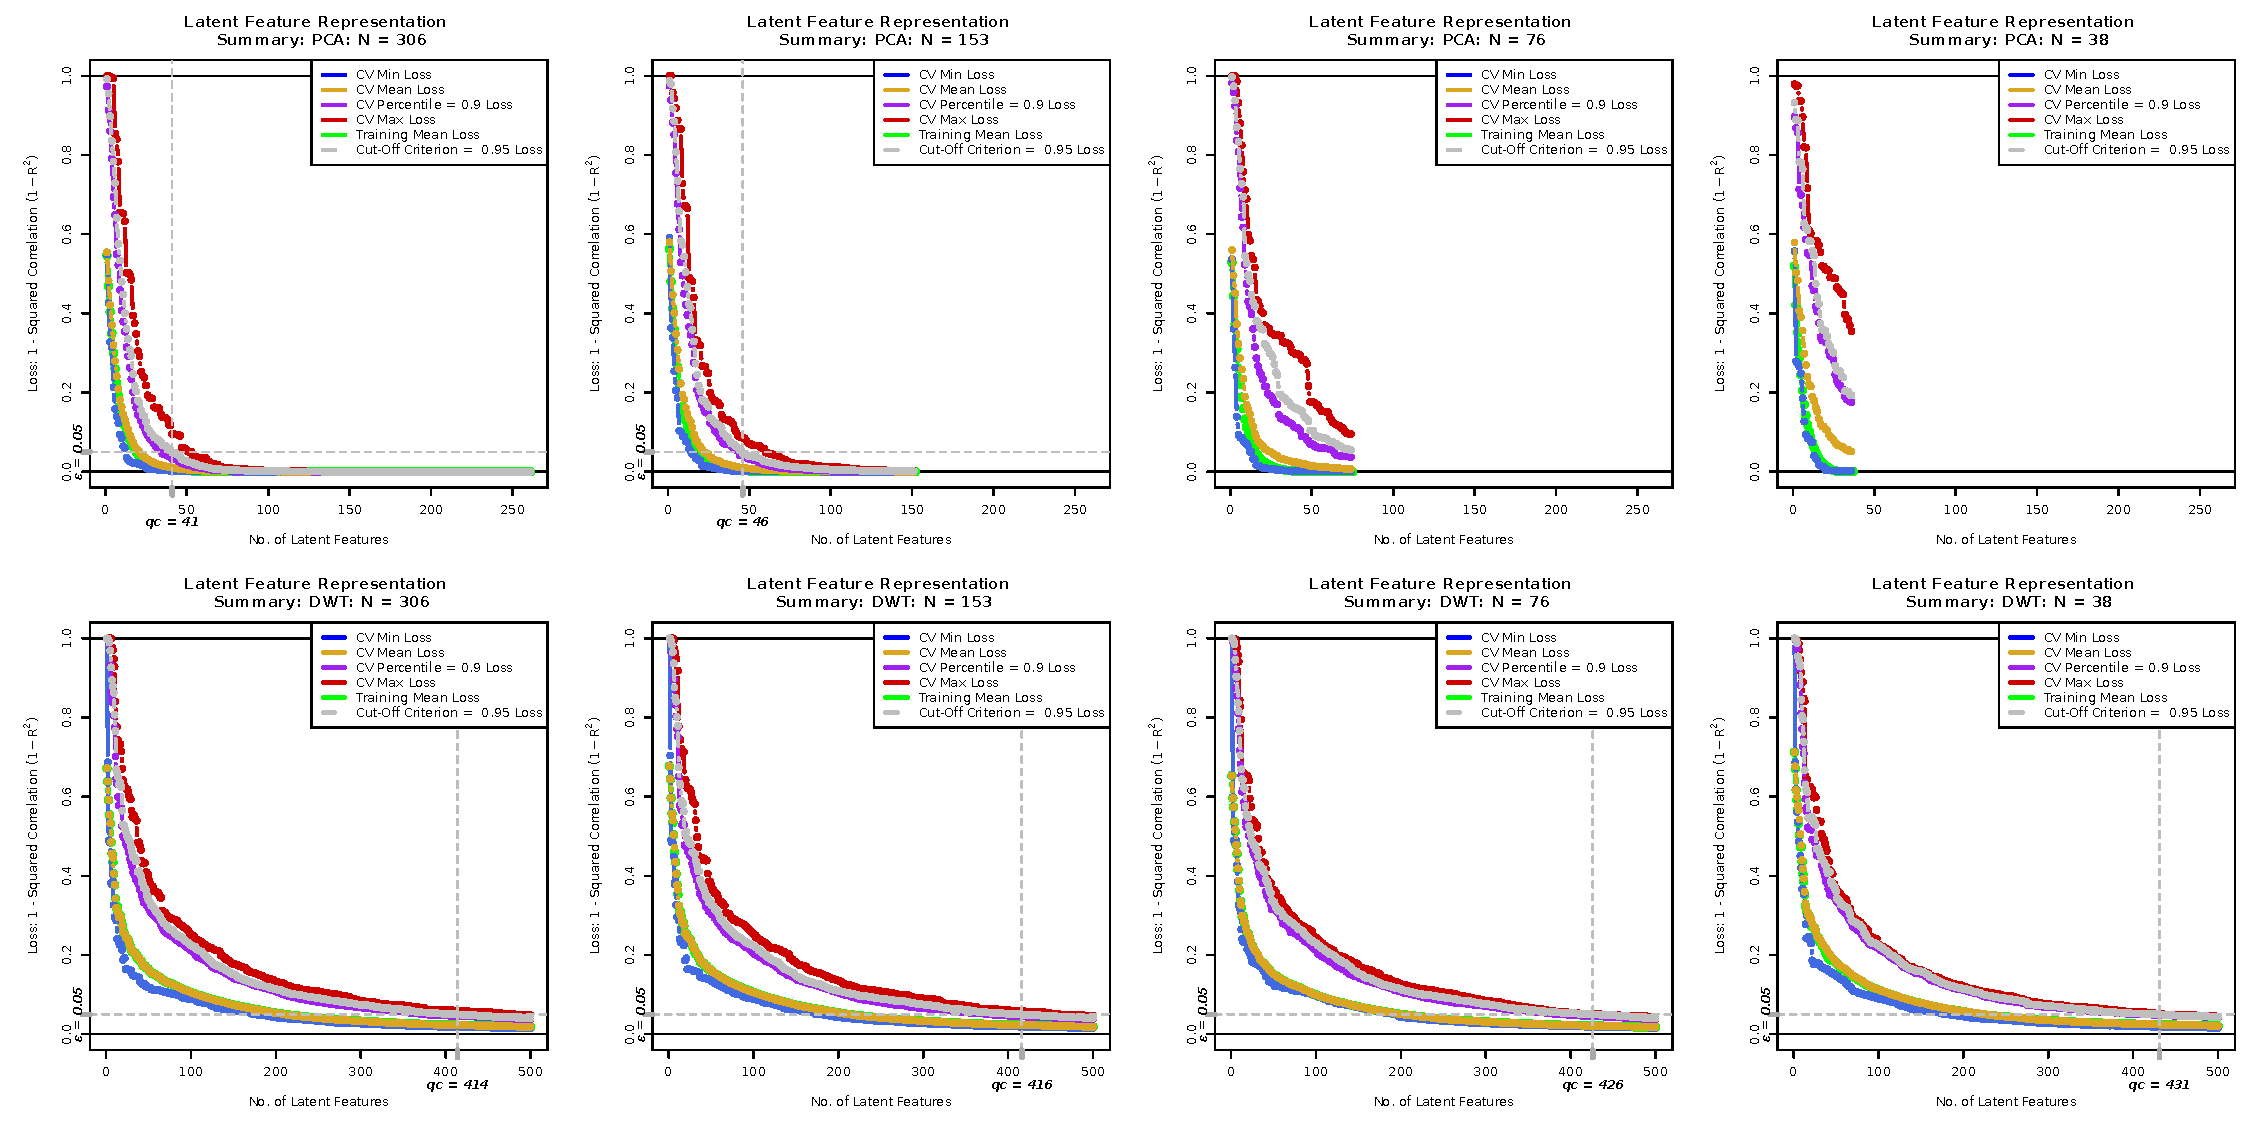
\includegraphics[width=1\linewidth]{figures/eye-sample-size-results-results-01.pdf}
    \caption{Results of the experiment to assess the affect of sample size on different latent feature representations. The Glaucoma data was used to create smaller datasets of size $N=153$, $N=76$ and $N=38$. \texttt{GLaRe()} was used to compare the representations provided by PCA (first row) and DWT (second row) as the sample size was decreased. Leave-one-out cross-validation was used in all cases.}
    \label{fig:eye-sample-size-results-results-01}
\end{figure}


